% case name
\chapter{Wind forced channel flow (stratif\_wind)}
%
% - Purpose & Description:
%     These first two parts give reader short details about the test case,
%     the physical phenomena involved, the geometry and specify how the numerical solution will be validated
%
\section{Purpose}
%
This test case belongs to a benchmark of CFD codes with analytical solutions.
Its aim was to study the behavior of different codes, focusing on situations
where the density variations have a crucial influence on the hydrodynamical
process.
This study was carried out during Lamia Abbas's post-doctoral \cite{Abbas2015}
in 2014-2015.

This test case demonstrates the ability of \telemac{3D} to simulate the response
of a density-stratified water to wind stress.
It is inspired by \cite{Audusse2011} and \cite{Pelanti}.
It models the wind blowing on a stratified lake.
The wind generates the defletion of the thermocline and 2 recirculations.
The example only shows the results for one specific 2D mesh and one distribution
of planes over the vertical.

%
\section{Description}
%
A 10~m long and 2~m wide channel with flat bottom (elevation $z$ = 0~m) is
considered.

The tracer used is temperature.
The density is considered as a function of the water temperature:
\begin{equation}
  \rho(T) = \rho_0 \left(1 - \alpha (T-T_0)^2\right),
\end{equation}
where $\rho_0$ = 999.972~kg.m$^{-3}$, $T_0$ = 4~$^{\circ}$C
and $\alpha$ = 7.10$^{-6}$.

There are two layers of water with different temperatures.
As the density depends on water temperature, the initial state
is chosen nearly stable \emph{i.e.} the heavier fluid is below the lighter
as shown in Figure \ref{fig:stratif_wind:temp_ic:section}.

%
\section{Computational options}
%
\subsection{Mesh}
%
The triangular mesh is made of 4,548 triangular elements (element size
$\approx$ 0.1~m) and 2,409 nodes (see Figure \ref{fig:stratif_wind:mesh}).

\begin{figure}[H]
 \centering
 \includegraphicsmaybe{[width=0.9\textwidth]}{../img/res_mesh.png}
  \caption{Horizontal mesh.}\label{fig:stratif_wind:mesh}
\end{figure}

To build the 3D mesh of prisms, 40 planes are regularly spaced over the vertical
(classical $\sigma$ transformation).
The vertical mesh between nodes of coordinates (0 ; 1) to (10 ; 1) can be seen
in Figure \ref{fig:stratif_wind:mesh:section}.

\begin{figure}[H]
 \centering
 \includegraphicsmaybe{[width=0.9\textwidth]}{../img/res_mesh_section.png}
  \caption{Vertical mesh.}\label{fig:stratif_wind:mesh:section}
\end{figure}

During Lamia Abbas's post-doctoral, one finer 2D grid was also used
($dl \approx$ 0.05~m) with 18,922 triangular elements and 9,721 nodes.

Moreover, 2 different vertical distributions were tested:
\begin{itemize}
\item one coarser vertical distribution with 20 horizontal planes
  leading to $\approx$ 0.05~m vertical height,
\item one finer vertical distribution with 80 horizontal planes leading to
  $\approx$ 0.0125~m vertical height.
\end{itemize}

\subsection{Physical parameters}
%
The turbulent viscosities for both velocities and tracers are constant,
also both for horizontal and vertical directions.
$\nu_z$ = 0.01~m$^2$/s but no diffusion for velocity along horizontal directions.
$\nu_T$ = 0 for both horizontal and vertical directions.\\
%Turbulence model (both horizontal and vertical): constant model\\
%Anisotropic viscosity for tracer: 0~m$^2$/s\\

A constant wind blows with a wind magnitude = 10~m/s along $x$ with
\telkey{COEFFICIENT OF WIND INFLUENCE} = 1.25.10$^{-6}$.
\telkey{THRESHOLD DEPTH FOR WIND} = 0.1~m as the vertical planes
are close just below the free surface.
%
\subsection{Initial and Boundary Conditions}
%
%\subsubsection{Initial conditions}
%
The initial free surface elevation is 1 m with a fluid at rest.
%Flow at rest: Constant elevation (= 1~m) and no velocity\\
The initial temperature depends on elevation, defined by:
\begin{equation}
  T_0(x,y,z) = \left\{
  \begin{tabular}{rl}
    25 $^{\circ}$C & if $z \geq$ 0.5~m,\\
    8  $^{\circ}$C & else
  \end{tabular}
  \right.
\end{equation}
see Figure \ref{fig:stratif_wind:temp_ic:section}.

\begin{figure}[H]
 \centering
 \includegraphicsmaybe{[width=0.9\textwidth]}{../img/res_temp_IC_section.png}
  \caption{Initial condition for temperature.}\label{fig:stratif_wind:temp_ic:section}
\end{figure}

%
%\subsubsection{Boundary conditions}
%
There are only closed lateral boundaries with free slip condition and no
friction at the bottom.
%
\subsection{General parameters}
%
The time step is 0.25~s for a simulated period of 1,200~s.
%
\subsection{Numerical parameters}
%
The non-hydrostatic version of \telemac{3D} is used.
To solve the advection steps, the method of characteristics is chosen for the
velocities and the PSI-type MURD scheme for the temperature.
Other advection schemes give similar results with \telemac{3D}.
%
% - Results:
%     We comment in this part the numerical results against the reference ones,
%     giving understanding keys and making assumptions when necessary.
%
\section{Expected results}
%
%
%\subsubsection{Expected results}
%\subsubsection{Remarks}

Audusse and al. \cite{Audusse2011} derive an analytical solution at the
stationary regime under the following hypotheses:
\begin{itemize}
\item Hydrostatic pressure assumption,
\item Stationary equilibrium state,
\item $\nu_T = 0$, $\nu_H = 0$, $\nu_z \neq 0$,
\item Near the mid-length of the bassin it is assumed:
  \begin{equation}
  \frac{\partial u}{\partial x} =0, \quad \frac{\partial^2 u}{\partial x^2} =0 \quad \textrm{and} \quad w = 0.
  \end{equation}
\end{itemize}

Under these hypotheses, two recirculations with counter directions will appear,
see Figure \ref{fig:stratif_wind:scheme}.

\begin{figure}[H]
  \begin{center}
    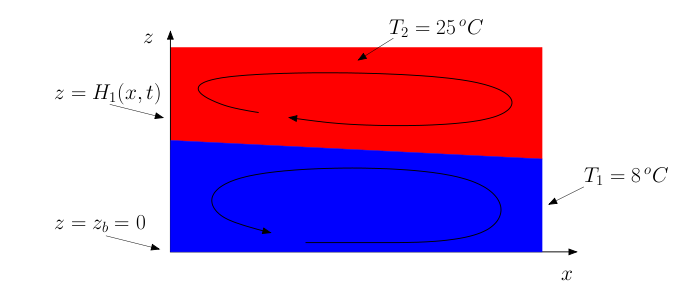
\includegraphics[width=15cm]{img/vent_ref}
    \caption{A schematical description of the solution (source \cite{Abbas2015}).}
    \label{fig:stratif_wind:scheme}
  \end{center}
\end{figure}

Moreover, the case where the initial location of the thermocline is
$H_1$ = $H$/2. 
Then, the velocities at the mid-length are:
%\begin{eqnarray*}
\begin{equation}
U_1(z) = \dfrac{H_1^2- 3 z^2}{12 \mu_1 H} \tau_s ,
\end{equation}

\begin{equation}
U_2(z) = \dfrac{15 z^2 + 36  H_1 z + 19 H_1^2}{12 \mu_2 H}\tau_s ,
\end{equation}
%\end{eqnarray*}
and the deflection of the thermocline is:
\begin{equation}
\frac{\partial H_1 }{\partial x} = \frac{\tau_s}{H(\rho_1-\rho_2)} .
\end{equation}

%\subsubsection{Required calculations}

\section{Results}

Figure \ref{fig:stratif_wind:temp:section} shows the final temperature
distribution (after 1,200~s) and the thermocline deflection.
As expected, the thermocline slope has the good sign, but due to the big
diffusion, it is difficult to compute it with accuracy.

\begin{figure}[H]
 \centering
 \includegraphicsmaybe{[width=0.9\textwidth]}{../img/res_temp_section.png}
  \caption{Temperature distribution after 1,200~s.}\label{fig:stratif_wind:temp:section}
\end{figure}

Figure \ref{fig:stratif_wind:velo_vectors:section} shows the final velocity
vectors (after 1,200~s) and the opposite circulations in the upper and the lower
layers.
%2 recirculations over the vertical.

%\begin{itemize}
%\item Temperature distribution to show the thermocline deflection,
%\item Velocity field (the opposite circulations in the upper and the lower layer),
\begin{figure}[H]
 \centering
%\includegraphics[width=7cm]{img/vent_telemach} \qquad
%\includegraphics[width=6.5cm]{img/vent_maillage5}
%\caption{\footnotesize Computation with TELEMAC-3D.}
\includegraphicsmaybe{[width=0.9\textwidth]}{../img/res_velocity_vectors_section.png}
\caption{Velocity field and vectors after 1,200~s.}\label{fig:stratif_wind:velo_vectors:section}
\end{figure}
%\item Comparison between the analytical and the computed velocities at the mid-length of the channel.
%not done yet, analytical solution to found
%\end{itemize}


See \cite{Abbas2015} for more informations, in particular the results for
different meshes and the comparision between the analytical and computed
velocities.

\section{Conclusion}
%
\telemac{3D} is able to simulate the response of a density-stratified water to
wind stress.
